\section{The Klinkenberg effect}

In 1941, L.J. Klinkenberg published a paper explaining discrepancies that was found in experiments when measuring the permeability for both liquids and gases in the same material\cite{klinkenberg1941permeability}. His discoveries were of great importance in the oil industry
\begin{aquote}{Klinkenberg, 1941}
	It has become common practice in the oil industry to determine the permeability of core material with dry air; the equipment usually employed for this determination is arranged to operate with the outlet of the sample at or near atmospheric pressure.
\end{aquote}
He introduced a linear scaling function $f_c(\text{Kn})$ that relates what he called the \textit{apparent permeability} $k_a$, the permeability measured in the lab for a fluid with arbitrary density, to the \textit{absolute permeability} $k_\infty$, the permeability for a liquid in the high density limit. The absolute permeability is a constant dependent only on the porous medium (which is the whole idea of the permeability). The relation is given as
\begin{align}
	k_a = f_c k_\infty = \left(1 + 4\alpha\frac{\lambda}{L}\right)k_\infty = \left(1 + 4\alpha\text{Kn}\right)k_\infty,
\end{align}
where $L$ is the diameter of the channel and $\alpha\approx 1.15$ is the no-slip factor in equation \eqref{eq:noslip_sliplength}. Since the mean free path is proportional to the inverse pressure, we can write the scaling function as
\begin{align}
	f_c = \left(1 + \frac{b}{\bar P}\right),
\end{align}
where $b$ is a constant depending on the material. In figure \ref{fig:klinkenberg_correction_factor}, we see that the Klinkenberg correction factor predicts a permeability that almost fifty times higher for a gas in a material with $\text{Kn}=10$. The figure also contains the Knudsen correction factor which is discussed in the next subsection. The Klinkenberg correction factor is derived using the first order slip velocity in equation \eqref{eq:linear_slip_velocity} which is not sufficient for high Knudsen numbers as we will see in section \ref{sec:results_for_simple_geometries}. Based on higher order slip velocity models, one can derive better permeability corrections. 
\begin{figure}[h]
\begin{center}
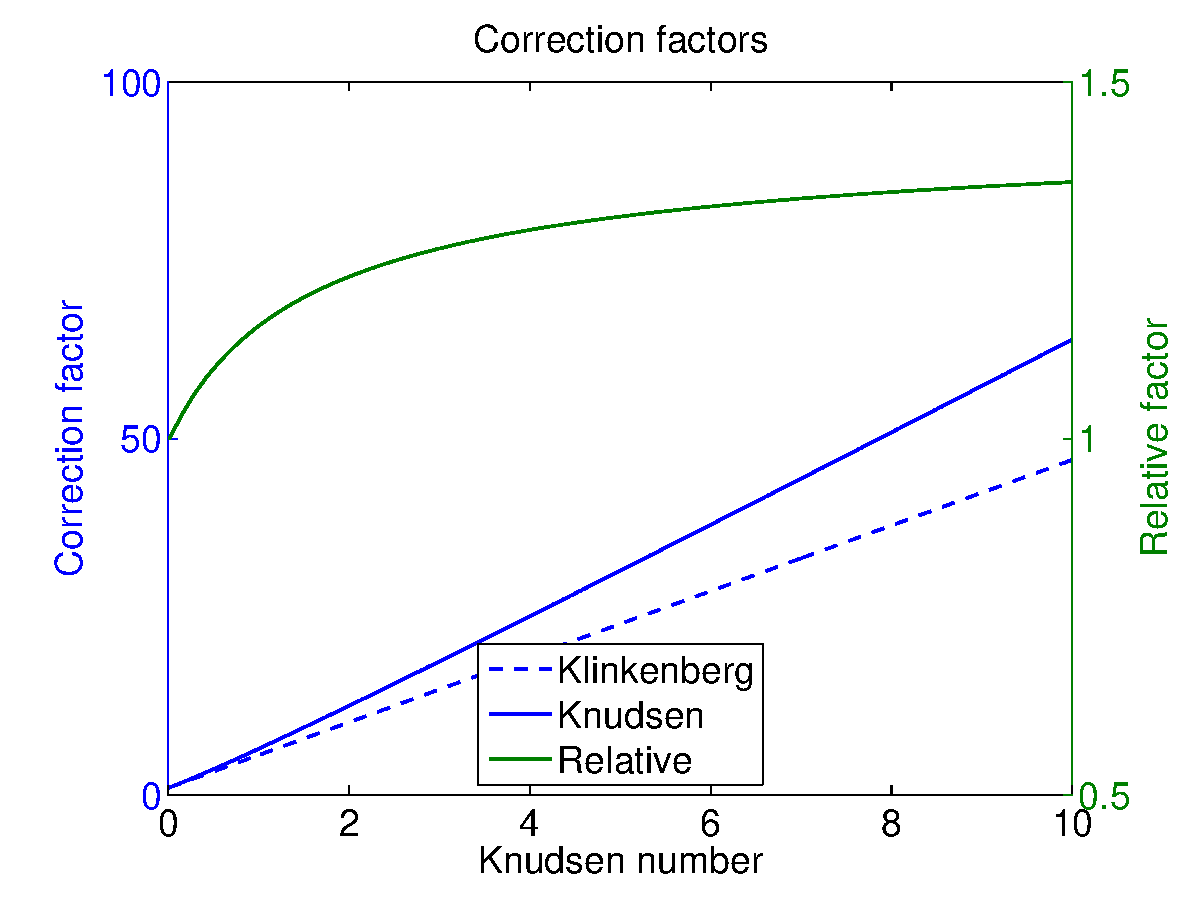
\includegraphics[width=\textwidth, trim=0cm 0cm 0cm 0cm, clip]{figures/klinkenberg.eps}
\end{center}
\caption{A comparison between the Klinkenberg factor and the Knudsen factor shows that slip velocity leads to even higher corrections to the permeability than what the Klinkenberg factor predicts. We see that in the high Knudsen number limit ($\text{Kn}=10$), we can expect an increase of permeability by a factor 50 compared to a liquid or a high density gas.}
\label{fig:klinkenberg_correction_factor}
\end{figure}

\section{Knudsen's correction}
\label{sec:knudsen_correction}
Beskok and Karniadakis (1999) developed another correction factor that uses a second order slip velocity model 
\begin{align}
	\label{eq:knudsen_correction}
	f_c = [1 + \alpha(\text{Kn})\text{Kn}]\left[1 + \frac{4\text{Kn}}{ 1 + \text{Kn}}\right],
\end{align}
where $\alpha(\text{Kn})$ is given as\cite{civan2010effective}
\begin{align}
	\alpha(\text{Kn}) = \frac{\alpha_0}{1 + \frac{A}{\text{Kn}^B}}
\end{align} 
where $A=0.170$, $B=0.4348$, and $\alpha_0=1.358$. These are fitted parameters based on a large dataset of Loyalka and Hamoodi (1990). We see in figure \ref{fig:klinkenberg_correction_factor} that the Knudsen factor predicts approximately 40\% higher correction than the Klinkenberg factor. In chapter \ref{chap:dsmc_results} we will check the validity of this correction factor for a simple cylinder, and discuss the practical problems we meet when studying flow in complex geometries where the system does not simply have one Knudsen number but rather a distribution of Knudsen numbers.